\documentclass[12pt]{scrartcl}
\input{../styles/Packages.tex}
\input{../styles/FormatAndHeader.tex}
\usepackage{tikz}

\usetikzlibrary{positioning}
\tikzset{
node of list/.style = { 
             draw, 
             fill=orange!20, 
             minimum height=6mm, 
             minimum width=6mm,
             node distance=6mm
   },
link/.style = {
     -stealth,
     shorten >=1pt
     },
array element/.style = {
    draw, fill=white,
    minimum width = 6mm,
    minimum height = 10mm
  }
}

\def\LinkedList#1{%
  \foreach \element in \list {
     \node[node of list, right = of aux, name=ele] {\element};
     \draw[link] (aux) -- (ele);
     \coordinate (aux) at (ele.east);
  } 
}
\usepackage{graphicx}

\setcounter{sheetnr}{7} % Nummer des Übungsblattes
\setcounter{exnum}{1} % Nummer der Aufgabe

% Beginn des eigentlichen Dokuments

\begin{document}

% Aufgabe 1
\exercise{Tiefensuche}
\begin{enumerate}
  \item Eingangsgrad und Ausgangsgrad
  \begin{center}
    \begin{tabular}{ |c|c|c|c| } 
     \hline
     Knoten & Eingangsgrad & Ausgangsgrad & Typ\\ \hline
     A & 0 & 1 & Quelle\\ \hline
     B & 2 & 2 & \\ \hline
     C & 0 & 2 & Quelle\\ \hline
     D & 2 & 3 & \\ \hline
     E & 0 & 2 & Quelle\\ \hline
     F & 3 & 1 & \\ \hline
     G & 2 & 1 & \\ \hline
     H & 3 & 0 & Senke\\
     \hline
    \end{tabular}
  \end{center}
  
  \item Tiefensuche
  \begin{enumerate}
    \item Startknoten $E$: H, G, E
    \item Startknoten $C$: H, D, B, F, G, C
    \item Startknoten $A$: F, B, H, D, A
  \end{enumerate} 

\end{enumerate}

\exercise{Topologische Sortierung}
\begin{enumerate}
  \item Topologische Sortierung: Suche die Reihenfolge der Knoten, so dass jeder Knoten nach all seinen Vorgngern kommt und es keine Zyklen gibt.
  \item Nein. Topologische Sortierung DFS benutzt. Wenn es für den Graph mehrere Quelle gibt, kann DFS beliebig mit einer der Startknoten starten. Deswegen gibt es die
  verschiedene Reihenfolge für DFS. Deshalb wird topologische Sortierung nicht eindeutig.
  \item Graph $G_2$
  \begin{enumerate}
    \item $G_2$
    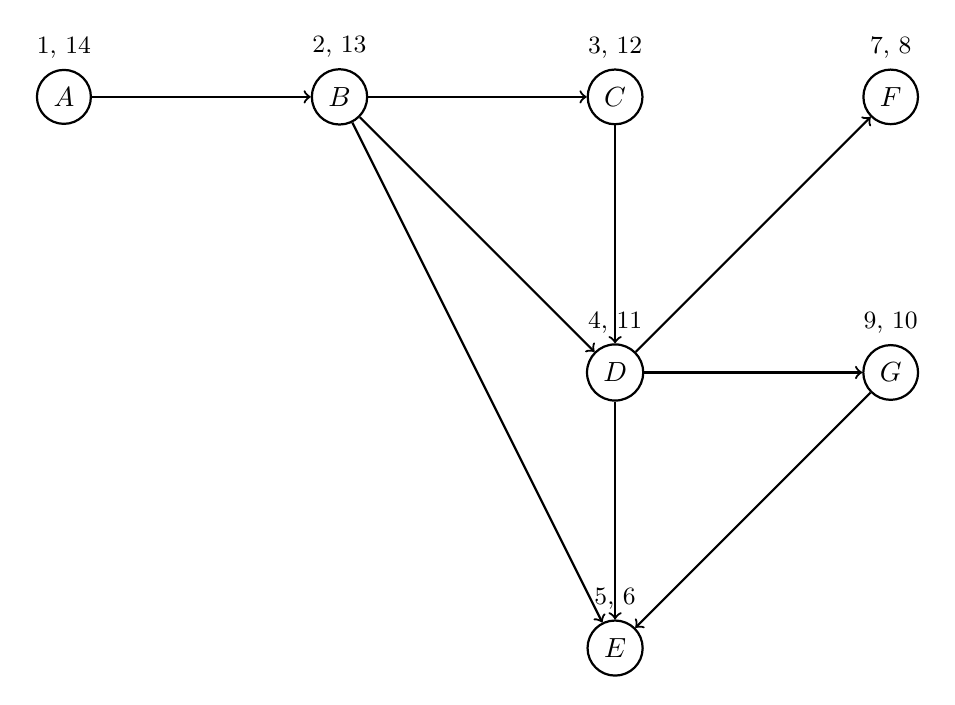
\begin{tikzpicture}[node distance={35mm}, thick, main/.style = {draw, circle}] 
      \node[main, label={\small 1, 14}] (1) {$A$}; 
      \node[main, label={\small 2, 13}] (2) [right of=1] {$B$}; 
      \node[main, label={\small 3, 12}] (3) [right of=2] {$C$}; 
      \node[main, label={\small 4, 11}] (4) [below of=3] {$D$}; 
      \node[main, label={\small 5, 6}] (5) [below of=4] {$E$}; 
      \node[main, label={\small 7, 8}] (6) [right of=3] {$F$};
      \node[main, label={\small 9, 10}] (7) [right of=4] {$G$};
      \draw[->] (1) -- (2) ; 
      \draw[->] (2) -- (3) ;
      \draw[->] (3) -- (4) ;
      \draw[->] (4) -- (5) ;
      \draw[->] (2) -- (4) ;
      \draw[->] (2) -- (5) ;
      \draw[->] (4) -- (6) ;
      \draw[->] (4) -- (7) ;
      \draw[->] (7) -- (5) ;
    \end{tikzpicture} 
    \item Ergebnisliste: 14 A -> 13 B -> 12 C -> 11 D -> 10 G -> 8 F -> 6 E
  \end{enumerate}
  \item Keine Änderung. Topologische Sortierung benutzt DFS. Wenn die Kante (E,B) hinzugefügt wird, gibt es keine Änderung für die Ergebnisliste. Da Knoten B bereits besucht ist.
\end{enumerate}

\setcounter{exnum}{4} % Nummer der Aufgabe
\exercise{Euler, Hamilton und kürzeste Wege}
\begin{enumerate}
  \item Graph $G_3$
  \begin{enumerate}
    \item Nein, mehr als zwei Knoten, z.B. Knoten$B, C, D, E, G$, haben einen ungeraden Grad.
    \item Nein, es gibt die Knoten, die einen ungeraden Grad haben.
    \item Ja, wie z.B. A->B->H->G->C->D->F->E
  \end{enumerate}
  \item Graph $G_4$\\
  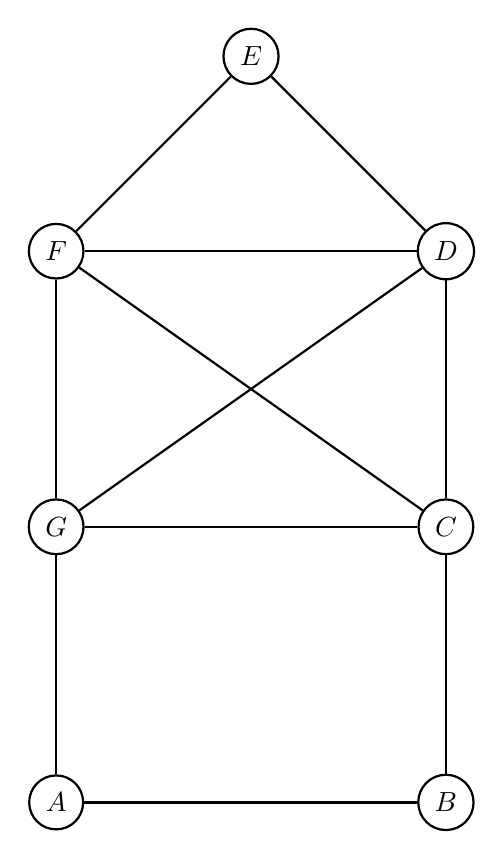
\begin{tikzpicture}[node distance={35mm}, thick, main/.style = {draw, circle}] 
    \node[main] (5) {$E$}; 
    \node[main] (6) [below left of=5] {$F$}; 
    \node[main] (4) [below right of=5] {$D$}; 
    \node[main] (7) [below of=6] {$G$}; 
    \node[main] (3) [below of=4] {$C$}; 
    \node[main] (1) [below of=7] {$A$};
    \node[main] (2) [below of=3] {$B$};
    \draw[-] (5) -- (6) ; 
    \draw[-] (5) -- (4) ;
    \draw[-] (6) -- (4) ;
    \draw[-] (6) -- (7) ;
    \draw[-] (4) -- (3) ;
    \draw[-] (7) -- (3) ;
    \draw[-] (6) -- (3) ;
    \draw[-] (7) -- (4) ;
    \draw[-] (7) -- (1) ;
    \draw[-] (1) -- (2) ;
    \draw[-] (2) -- (3) ;
  \end{tikzpicture}
  \begin{enumerate}
    \item Ja, alle Knoten haben einen geraden Grad.
    \item Ja, die Antwort verändert sich. Auf diesem Fall haben die Knoten A und B den ungeraden Grad 3. Deswegen gibt es keinen Euler'schen Kreis.
  \end{enumerate}
  \item Im Graph $G_5$ gibt es die Kanten, wie z.B. (c,g) = -3 und (e, c) = -1, die negativen Gewicht haben.
\end{enumerate}
\end{document}
